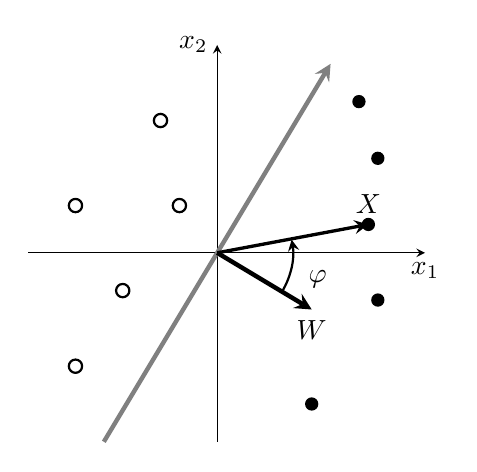
\begin{tikzpicture}[
  scale=1.2,
  arrow/.style = {->,>=stealth}]
  % osi
  \draw[arrow, black] (-2,0) -- (2.2,0) node[below] {$x_1$};
  \draw[arrow, black] (0,-2) -- (0,2.2) node[left] {$x_2$};

  % trieda 1 - krúžky
  \foreach \x/\y in {-1.5/0.5, -0.6/1.4, -0.4/0.5, -1.5/-1.2, -1.0/-0.4}
    \draw[thick] (\x,\y) circle (2 pt);

  % trieda 2 - plné krúžky
  \foreach \x/\y in {1.6/0.3, 1.5/1.6, 1.7/1.0, 1.7/-0.5, 1.0/-1.6}
    \fill (\x,\y) circle (2 pt);

  % rozhodovacia hranica
  \draw[arrow, gray, ultra thick] (-1.2,-2.0) -- (1.2,2.0);

  % súradnice vektorov
  \coordinate (O) at (0,0);
  \coordinate (X) at (1.6, 0.3);
  \coordinate (W) at (1.0, -0.6);

  % vektory
  \draw[arrow, black, very thick] (O) -- (X) node[above] {$X$};
  \draw[arrow, black, ultra thick] (O) -- (W) node[below] {$W$};

  % uhol
  % \draw [arrow, thick, black] 
  % \pic [draw] {angle = W--O--X};

  \draw[arrow, thick] (O) ++(-31:0.8cm) arc[start angle=-31, end angle=10, radius=0.8cm];
  \node at (-15:1.1cm) {$\varphi$};

\end{tikzpicture}